\documentclass[8pt, letterpaper]{article}
\usepackage[ngerman]{babel}
\usepackage{graphicx}
\usepackage[utf8]{inputenc}
\usepackage{gensymb}
\usepackage{blindtext}
\usepackage{geometry}
\usepackage{fancyhdr}
\usepackage{url}
\usepackage{seqsplit}
\usepackage{hyperref}

\graphicspath{{images/}}
\setlength{\parindent}{0cm}
\bibliographystyle{gerplain}
\geometry{letterpaper, margin=1in}
\pagestyle{fancy}

\lhead{Jakob Kirsch}
\rhead{
\includegraphics[width=3cm]{logo}}

\title{}
\author{Jakob Kirsch}
\date{\parbox{\linewidth}{\centering%
  \today\endgraf\bigskip
  Fach: IT\endgraf\medskip
  Betreuer: Herr Kutzner\endgraf\medskip
}}

\begin{document}

\maketitle
\newpage

\section{Aufgabenstellung}
Es sollen die Stromstaerke und Spannung eines Arduino UNOs und eventuelle Peripherien gemessen werden, um deren Verbrauch zu messen.
Uns wurden 4 verschiedene Szenarien gegeben:

\begin{enumerate}
  \item Im laufenden Betrieb ohne zusaetzliche Bauteile
  \item Im laufenden Betrieb mit einer leuchtenden roten LED
  \item Im laufenden Betrieb mit einer leuchtenden blauen LED
  \item Im laufenden Betrieb mit einem Servomotor in staendiger Bewegung
\end{enumerate}

\section{Versuchsmaterial}
\begin{itemize}
  \item Arduino UNO
  \item Breadboard
  \item diverse Kabel fuer das Breadboard und den Arduino UNO
  \item 9V Batterie
  \item Digitalmultimeter
  \item Klemmen fuer das Digitalmultimeter
  \item Widerstaende fuer die LEDs
  \item rote LED
  \item blaue LED
  \item Servomotor
\end{itemize}

\section{Messchaltungen}
\subsection{Spannungsmessung}
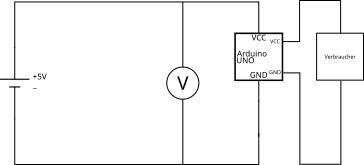
\includegraphics[width=9cm]{volt}
\subsection{Stromstaerkemessung}
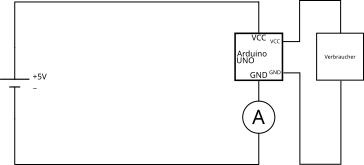
\includegraphics[width=9cm]{ampere}

\section{Messwerte}
\begin{center}
\begin{tabular}{ |c|c|c|c|c| }
  Messgoesse & ohne Baugruppen & mit roter LED & mit blauer LED & mit Servomotor \\
  \hline
  Spannung [V] & & & & \\
  \hline
  Stromstaerke [mA] & & & & \\
  \hline
  Leistung rechn. [mW] & & & & \\
  \hline
\end{tabular}
\end{center}

\section{Evtl. Beobachtungen}
Bei jedem Aufbau schwanken die Werte sehr, wodurch man warten muss, bis diese sich halbwegs stabilisieren. Das liegt wahrscheinlich an verschiedenen Bauteilen, wie Kondensatoren.

\section{Berechnung}

\break

\section{Auswertung}

\end{document}
